% Gabarit pandoc des corrigés publiés (brut et guidé). Contenu sans marque ni nom de site.
% Compilation : lualatex (latexmk -lualatex).
% Le Markdown reste la source unique : ne pas éditer ce fichier .tex à la main.
\documentclass[11pt,a4paper]{article}

% --- Moteur, polices (Latin Modern) et langue ---------------------------------
\usepackage{iftex}
\ifLuaTeX\else\errmessage{Ce document se compile avec lualatex}\fi
\usepackage{amsmath,amssymb,mathtools}
\usepackage{fontspec}
% mathrm=sym : \mathrm prend ses glyphes dans la police mathématique (ℓ, μ, Ω), comme KaTeX.
\usepackage[math-style=TeX,bold-style=TeX,mathrm=sym]{unicode-math}
% Repli pour les glyphes absents de Latin Modern (indices et exposants Unicode,
% flèches, filets des schémas en texte, symboles) : DejaVu, puis Latin Modern Math
% (ℓ, lettres mathématiques Unicode des légendes).
\directlua{
  luaotfload.add_fallback("repliTexte", {"DejaVuSerif:mode=harf;", "DejaVuSans:mode=harf;", "file:latinmodern-math.otf:mode=harf;"})
  luaotfload.add_fallback("repliMono", {"DejaVuSansMono:mode=harf;", "DejaVuSans:mode=harf;", "file:latinmodern-math.otf:mode=harf;"})
}
\setmainfont{Latin Modern Roman}[RawFeature={fallback=repliTexte}]
\setsansfont{Latin Modern Sans}[RawFeature={fallback=repliTexte}]
\setmonofont{Latin Modern Mono}[RawFeature={fallback=repliMono}]
\setmathfont{Latin Modern Math}
\usepackage[french]{babel}
\frenchsetup{SmallCapsFigTabCaptions=false}

% --- Mise en page --------------------------------------------------------------
\usepackage[a4paper,margin=2.2cm,headheight=14pt,footskip=1.2cm]{geometry}
\usepackage{microtype}
\setlength{\emergencystretch}{4em}
\tolerance=1500
\setlength{\parindent}{0pt}
\setlength{\parskip}{0.55\baselineskip plus 2pt minus 1pt}
\usepackage{xcolor}
% Gris nommés : babel-french rend « ! » actif dans le document.
\definecolor{gris2}{gray}{0.98}
\definecolor{gris3}{gray}{0.97}
\definecolor{gris5}{gray}{0.95}
\definecolor{gris35}{gray}{0.65}
\definecolor{gris40}{gray}{0.60}
\definecolor{gris45}{gray}{0.55}
\definecolor{gris50}{gray}{0.50}
\definecolor{gris55}{gray}{0.45}
\definecolor{gris60}{gray}{0.40}
\definecolor{gris65}{gray}{0.35}
\definecolor{gris70}{gray}{0.30}
\definecolor{gris80}{gray}{0.20}
\definecolor{gris85}{gray}{0.15}
\usepackage{graphicx}
\usepackage{float}
\usepackage{caption}
\captionsetup{font=small,labelformat=empty,justification=centering}
\usepackage{booktabs,longtable,array,multirow,calc}
\usepackage{siunitx}
\sisetup{locale=FR}
\usepackage[version=4]{mhchem}
\usepackage{listings}
\usepackage{fancyhdr}
\usepackage{lastpage}
\usepackage[most]{tcolorbox}
\usepackage{enumitem}
\setlist{nosep,leftmargin=*,topsep=2pt}
\usepackage[hidelinks,unicode]{hyperref}
\usepackage{bookmark}
\hypersetup{pdftitle={e3a-Polytech PC — Mathématiques 2026},pdfauthor={Rédigé par IA},pdfcreator={LaTeX},pdfsubject={Corrigé guidé}}
\usepackage{xurl}

% --- Pandoc : listes, tableaux, figures ----------------------------------------
\providecommand{\passthrough}[1]{#1}
\providecommand{\tightlist}{\setlength{\itemsep}{0pt}\setlength{\parskip}{0pt}}

\makeatletter
\def\maxwidth{\ifdim\Gin@nat@width>\linewidth\linewidth\else\Gin@nat@width\fi}
\def\maxheight{\ifdim\Gin@nat@height>0.55\textheight 0.55\textheight\else\Gin@nat@height\fi}
\makeatother
\setkeys{Gin}{width=\maxwidth,height=\maxheight,keepaspectratio}
\setcounter{secnumdepth}{-\maxdimen}
\providecommand{\pandocbounded}[1]{#1}
\usepackage{longtable,booktabs,array}

% --- Code (listings) -----------------------------------------------------------
\lstset{
  basicstyle=\ttfamily\small,
  columns=fullflexible,
  keepspaces=true,
  breaklines=true,
  breakatwhitespace=false,
  postbreak=\mbox{\textcolor{gris50}{$\hookrightarrow$}\space},
  frame=single,
  rulecolor=\color{gris35},
  framesep=4pt,
  xleftmargin=5pt,xrightmargin=5pt,
  backgroundcolor=\color{gris3},
  keywordstyle=\bfseries,
  commentstyle=\color{gris65},
  stringstyle=\color{gris80},
  showstringspaces=false,
  tabsize=4,
  extendedchars=true,
  aboveskip=6pt,belowskip=6pt,
}

% --- Macros des corrigés (KaTeX ↔ LaTeX) ---------------------------------------
% Les corrigés sont écrits pour KaTeX : on définit ici ce que KaTeX connaît et
% que LaTeX n'a pas, sans jamais retoucher le Markdown.
\providecommand{\R}{\mathbb{R}}
\providecommand{\N}{\mathbb{N}}
\providecommand{\Z}{\mathbb{Z}}
\providecommand{\Q}{\mathbb{Q}}
\providecommand{\C}{\mathbb{C}}
\providecommand{\dd}{\mathrm{d}}
\providecommand{\llbracket}{\lBrack}
\providecommand{\rrbracket}{\rBrack}
\providecommand{\lBrace}{\lbrace}
\providecommand{\rBrace}{\rbrace}
\providecommand{\Box}{\square}
\providecommand{\Diamond}{\lozenge}
\providecommand{\varnothing}{\emptyset}
\providecommand{\argmax}{\operatorname*{arg\,max}}
\providecommand{\argmin}{\operatorname*{arg\,min}}
\renewcommand{\leq}{\leqslant}
\renewcommand{\geq}{\geqslant}

% Équation hors texte : réduite à la largeur de la ligne si elle déborde.
\newsavebox{\boiteequation}
\newcommand{\equationajustee}[1]{%
  \sbox{\boiteequation}{$\displaystyle #1$}%
  \ifdim\wd\boiteequation>\linewidth
    \[\resizebox{\linewidth}{!}{\usebox{\boiteequation}}\]%
  \else
    \[#1\]%
  \fi}

% --- Encadrés pédagogiques (sobres, lisibles en noir et blanc) -----------------
\tcbset{
  encadre/.style={
    enhanced,breakable,sharp corners,
    colback=white,colframe=gris55,
    boxrule=0.4pt,leftrule=2.2pt,
    left=6pt,right=6pt,top=3pt,bottom=3pt,
    before skip=6pt,after skip=6pt,
    fonttitle=\bfseries\small,coltitle=black,
    attach title to upper,after title={\quad},
    parbox=false,
  }
}
\newtcolorbox{indication}[1]{encadre,colframe=gris45,colback=gris2,title={Indication~#1}}
\newtcolorbox{methode}{encadre,colframe=gris70,title={Méthode}}
\newtcolorbox{piege}{encadre,colframe=gris85,boxrule=0.8pt,leftrule=2.2pt,title={Piège}}
\newtcolorbox{jury}{encadre,colframe=gris60,colback=gris5,title={Jury}}
\newtcolorbox{encadrenote}{encadre,colframe=gris40}

% --- Titres de section ---------------------------------------------------------
\usepackage{titlesec}
\titleformat{\section}{\Large\bfseries}{}{0pt}{}
\titleformat{\subsection}{\large\bfseries}{}{0pt}{}
\titleformat{\subsubsection}{\normalsize\bfseries}{}{0pt}{}
\titlespacing*{\section}{0pt}{14pt plus 4pt minus 2pt}{6pt}
\titlespacing*{\subsection}{0pt}{10pt plus 3pt minus 2pt}{4pt}
\titlespacing*{\subsubsection}{0pt}{8pt plus 2pt minus 2pt}{2pt}

% --- En-tête et pied de page ---------------------------------------------------
\pagestyle{fancy}
\fancyhf{}
\fancyhead[L]{\small\textsc{Corrigé guidé} · e3a-Polytech PC}
\fancyhead[R]{\small Maths 2026}
\fancyfoot[L]{\footnotesize Corrigé rédigé par IA, non officiel}
\fancyfoot[R]{\footnotesize \thepage\,/\,\pageref*{LastPage}}
\renewcommand{\headrulewidth}{0.4pt}
\renewcommand{\footrulewidth}{0pt}
\fancypagestyle{plain}{\fancyhf{}\fancyfoot[R]{\footnotesize \thepage\,/\,\pageref*{LastPage}}\fancyfoot[L]{\footnotesize Corrigé rédigé par IA, non officiel}\renewcommand{\headrulewidth}{0pt}}

\begin{document}
\thispagestyle{plain}
\begin{center}
  {\small\scshape Corrigé guidé}\par\smallskip
  {\LARGE\bfseries e3a-Polytech PC — Mathématiques 2026\par}\medskip
  {\large e3a-Polytech · PC · Maths · 2026\par}
\end{center}
\vspace{2pt}\hrule\vspace{8pt}

\emph{Corrigé rédigé par IA, non officiel. Signalez toute erreur.}

\hypertarget{pruxe9sentation-du-sujet}{%
\section{Présentation du sujet}\label{pruxe9sentation-du-sujet}}

L'épreuve (code PC8M) dure \textbf{4 heures}, sans calculatrice ni document. Elle comporte \textbf{trois exercices indépendants}, soit \textbf{42 questions} courtes et très guidées.

Chaque exercice suit le même schéma : des questions préliminaires de cours isolent les outils, puis un exemple les met en œuvre. Le sujet ne contient aucun piège technique lourd : la note se joue sur la \textbf{rigueur des justifications} (vecteur propre non nul, hypothèses des théorèmes, intervalle de travail) et sur la \textbf{propreté des calculs}.

\begin{longtable}[]{@{}
  >{\raggedright\arraybackslash}p{(\columnwidth - 6\tabcolsep) * \real{0.1776}}
  >{\raggedright\arraybackslash}p{(\columnwidth - 6\tabcolsep) * \real{0.1879}}
  >{\raggedright\arraybackslash}p{(\columnwidth - 6\tabcolsep) * \real{0.3096}}
  >{\raggedright\arraybackslash}p{(\columnwidth - 6\tabcolsep) * \real{0.2950}}@{}}
\toprule\noalign{}
\begin{minipage}[b]{\linewidth}\raggedright
Exercice
\end{minipage} & \begin{minipage}[b]{\linewidth}\raggedright
Questions
\end{minipage} & \begin{minipage}[b]{\linewidth}\raggedright
Contenu
\end{minipage} & \begin{minipage}[b]{\linewidth}\raggedright
Notions du programme PC
\end{minipage} \\
\midrule\noalign{}
\endhead
\bottomrule\noalign{}
\endlastfoot
1 -- Un endomorphisme antisymétrique de \(\mathbb R^5\) & 1--4, 5.1--5.6, 6.1--6.3, 7, 8.1, 8.2, 9, 10 (18 questions) & \(M^\top=-M\) : \(f\) non inversible, non diagonalisable, \(f^2\) symétrique ; \(E=\operatorname{Ker}f\oplus\operatorname{Im}f\) ; base adaptée formée de plans stables. & Déterminant, rang, éléments propres, somme directe, espaces euclidiens, endomorphismes symétriques, théorème spectral, matrices semblables \\
2 -- Une transformation intégrale & 1--3, 4, 5.1--5.4, 6.1, 6.2.1--6.2.3 (12 questions) & \(F(x)=\int_0^1\frac{f(t)}{x+t}dt\) : formule exacte pour \(f(t)=t^n\), puis pour \(f=\exp\), régularité, limite et équivalent en \(0^+\). & Développements limités, théorème fondamental de l'analyse, changement de variable, prolongement par continuité, relations de comparaison \\
3 -- Variance extrémale & 1--3, 4.1--4.7, 5, 6 (12 questions) & La variance d'une variable à valeurs dans \(\{1,2,3\}\) est une fonction de deux variables sur un triangle ; extrema atteints sur le bord. & Espérance, formule de transfert, variance, fonctions de deux variables, gradient, points critiques, théorème des bornes atteintes \\
\end{longtable}

\textbf{Difficulté.} Les questions sont de niveau modeste prises une à une, mais le sujet est long à rédiger proprement, et le résultat de la session est faible.

Le rapport 2026 donne une moyenne de 6,41 sur 20 (écart type 3,13, sur 2341 copies) et juge le bilan « assez mitigé avec très peu de bonnes copies ». Les points qui demandent de l'attention :

\begin{itemize}
\tightlist
\item
  Ex. 1, Q2 et Q8.1 : vérifier qu'un vecteur propre est \textbf{non nul}, et exploiter le \textbf{signe} de \(\lambda\) ;
\item
  Ex. 1, Q9 : combiner trois résultats antérieurs pour obtenir une famille libre ;
\item
  Ex. 2, Q5.3 : un calcul de signes avec les puissances de \(-x\) ;
\item
  Ex. 2, Q6.2.2 : une dérivation où tout doit se simplifier exactement ;
\item
  Ex. 3, Q4.7 : justifier que les extrema sont sur le bord, puis étudier les \textbf{trois} côtés.
\end{itemize}

\textbf{Questions discriminantes selon le rapport 2026.} Le rapport ne donne pas de taux par question, mais ses commentaires désignent nettement les questions qui ont fait la différence :

\begin{itemize}
\tightlist
\item
  Ex. 1, Q7 (« peu de réussite pour cette question classique »), Q8.1, Q9 et Q10 (« rarement abordée et rarement aboutie ») ;
\item
  Ex. 2, Q2, qualifiée de « fiasco total », puis Q6.1, Q6.2.2 et Q6.2.3 (« quasiment jamais achevée ») ;
\item
  Ex. 3, Q4.4 (gradient), Q4.6 et Q4.7, puis Q5 et Q6, rarement menées au bout.
\end{itemize}

\textbf{Questions abordables à ne pas laisser passer} : Ex. 1, Q1, 3, 4, 5.1 à 5.6 et 6.2 ; Ex. 2, Q1 à 4, 5.1, 5.2 et 6.1 ; Ex. 3, Q1 à 3 et 4.1 à 4.6.

Le jury signale qu'une partie non négligeable du barème porte sur la présentation : numérotation du sujet respectée, questions dans l'ordre, copie lisible.

\textbf{Gestion du temps.} Comptez environ 90 minutes pour l'exercice 1, le plus long, 75 minutes pour l'exercice 2 et 60 minutes pour l'exercice 3, et gardez 15 minutes de relecture.

Les trois exercices sont indépendants : commencez par celui qui vous inspire le plus. Dans l'exercice 1, les questions 7 à 10 n'utilisent que des résultats énoncés (dont le spectre admis de \(f^2\)) : on peut les traiter même si l'on a calé avant.

\begin{jury}

Le rapport 2026 rappelle que « une affirmation sans démonstration n'a aucune valeur » et conclut : « lire attentivement l'énoncé en étudiant toutes les interactions entre les questions reste d'une importance capitale pour réussir cette épreuve » (p.~2). Les questions préliminaires servent aux exemples : citez-les explicitement quand vous les utilisez.

\end{jury}

\hypertarget{exercice-1-un-endomorphisme-antisymuxe9trique-de-mathbb-r5}{%
\section{\texorpdfstring{Exercice 1 --- Un endomorphisme antisymétrique de \(\mathbb R^5\)}{Exercice 1 --- Un endomorphisme antisymétrique de \textbackslash mathbb R\^{}5}}\label{exercice-1-un-endomorphisme-antisymuxe9trique-de-mathbb-r5}}

Les préliminaires établissent quatre faits généraux sur les valeurs propres de \(g\) et \(g^2\) et sur les déterminants. On les applique ensuite à \(f\), dont la matrice vérifie \(M^\top=-M\).

Cette antisymétrie, traduite en \((f(x)\mid y)=-(x\mid f(y))\), est le seul ingrédient de presque toutes les preuves. On aboutit à une décomposition de \(E\) en une droite (le noyau) et deux plans stables, sur lesquels \(f\) agit comme une « rotation d'un quart de tour suivie d'une dilatation ».

\hypertarget{question-1}{%
\subsection{Question 1}\label{question-1}}

\begin{indication}{1}

Revenez à la définition : une valeur propre, c'est un vecteur non nul \(x\) tel que \(g(x)=\mu x\). Appliquez \(g\) une seconde fois.

\end{indication}

\hypertarget{solution}{%
\subsubsection{Solution}\label{solution}}

Soit \(\mu\) une valeur propre de \(g\). Il existe \(x\neq0\) tel que \(g(x)=\mu x\). Par linéarité de \(g\) :

\equationajustee{\begin{aligned}
g^2(x)&=g(\mu x)\\
&=\mu\,g(x)\\
&=\mu^2x.
\end{aligned}}

Comme \(x\neq0\), \textbf{\(\mu^2\) est valeur propre de \(g^2\)}, et \(x\) est un vecteur propre associé.

\begin{jury}

Rapport 2026 (p.~4) : « Le fait que \(x\) qui vérifie \(g(x)=\mu x\) est non nul est rarement évoqué. » Le jury relève aussi des confusions entre valeur propre et élément du noyau, du type « \(g(\mu)=0\) ». La non-nullité du vecteur propre doit figurer dans la copie.

\end{jury}

\hypertarget{question-2}{%
\subsection{Question 2}\label{question-2}}

\begin{indication}{1}

Calculez \(g^2(g(x))\) en faisant commuter \(g\) et \(g^2\).

\end{indication}

\begin{indication}{2}

Un vecteur propre doit être non nul : que se passerait-il si \(g(x)=0\) ? Utilisez l'hypothèse « valeur propre non nulle ».

\end{indication}

\hypertarget{solution-1}{%
\subsubsection{Solution}\label{solution-1}}

Soit \(x\neq0\) avec \(g^2(x)=\lambda x\) et \(\lambda\neq0\). On a :

\equationajustee{\begin{aligned}
g^2(g(x))&=g^3(x)\\
&=g(g^2(x))\\
&=g(\lambda x)\\
&=\lambda\,g(x).
\end{aligned}}

Il reste à voir que \(g(x)\neq0\). Si \(g(x)=0\), alors \(\lambda x=g^2(x)=g(0)=0\).

Comme \(\lambda\neq0\), on aurait \(x=0\) : contradiction. Donc \(g(x)\neq0\).

\textbf{\(g(x)\) est un vecteur propre de \(g^2\) associé à la même valeur propre \(\lambda\).}

\begin{piege}

Écrire seulement \(g^2(g(x))=\lambda g(x)\) ne suffit pas : c'est la non-nullité de \(g(x)\) qui fait de lui un vecteur propre. C'est précisément là que sert l'hypothèse \(\lambda\neq0\) : si \(\lambda=0\), \(g(x)\) peut être nul (prendre \(g\) nilpotent).

\end{piege}

\begin{piege}

Ne supposez pas que \(x\) est aussi vecteur propre de \(g\) : c'est faux en général, et c'est même exclu dans la suite (question 8.1). Le rapport 2026 (p.~4) note : « Il est assez fréquent que le candidat considère que \(x\) est aussi vecteur propre de \(g\). »

\end{piege}

\begin{jury}

Rapport 2026 (p.~4) : « Le fait que \(g(x)\) n'est pas le vecteur nul est rarement vérifié. »

\end{jury}

\hypertarget{question-3}{%
\subsection{Question 3}\label{question-3}}

\begin{indication}{1}

Pour \textbf{deux} sous-espaces, être en somme directe équivaut à avoir une intersection réduite à \(\{0\}\).

\end{indication}

\hypertarget{solution-2}{%
\subsubsection{Solution}\label{solution-2}}

Soient \(\mu_1\neq\mu_2\) deux valeurs propres de \(g\), et \(x\in E_{\mu_1}(g)\cap E_{\mu_2}(g)\).

Alors \(\mu_1x=g(x)=\mu_2x\), d'où \((\mu_1-\mu_2)x=0\).

Comme \(\mu_1-\mu_2\neq0\), on obtient \(x=0\).

L'intersection est réduite à \(\{0\}\), donc \textbf{les sous-espaces propres \(E_{\mu_1}(g)\) et \(E_{\mu_2}(g)\) sont en somme directe.}

\begin{piege}

Le critère « intersection nulle » ne vaut que pour deux sous-espaces. Pour trois sous-espaces ou plus, les intersections deux à deux nulles ne suffisent pas à garantir une somme directe.

\end{piege}

\begin{piege}

L'intersection de deux sous-espaces vectoriels contient toujours \(0\) : elle vaut \(\{0\}\), jamais \(\varnothing\). Le jury a lu « \(E_\lambda\cap E_\mu=\{\varnothing\}\) » dans des copies.

\end{piege}

\begin{jury}

Rapport 2026 (p.~4) : « Bien que cette question soit une question de cours, la réussite ne fut pas toujours au rendez-vous. »

\end{jury}

\hypertarget{question-4}{%
\subsection{Question 4}\label{question-4}}

\begin{indication}{1}

Le déterminant est linéaire par rapport à chacune des \(n\) colonnes.

\end{indication}

\hypertarget{solution-3}{%
\subsubsection{Solution}\label{solution-3}}

\equationajustee{\boxed{\det(-A)=(-1)^n\det(A)}}

\equationajustee{\boxed{\det(A^\top)=\det(A)}}

\begin{piege}

\(\det(-A)\) vaut \(-\det(A)\) seulement si \(n\) est impair ; pour \(n\) pair, \(\det(-A)=\det(A)\).

Le facteur \((-1)^n\) vient de ce qu'on sort un signe \(-1\) de chacune des \(n\) colonnes.

\end{piege}

\begin{jury}

Rapport 2026 (p.~4) : « Pour la grande majorité des candidats, \(\det(-A)=-\det(A)\). » Le jury cite aussi « \(\det(A^\top)=(\det(A))^\top\) », qui n'a pas de sens pour un nombre réel.

\end{jury}

\hypertarget{question-5-premiuxe8res-propriuxe9tuxe9s-de-lendomorphisme-f}{%
\subsection{\texorpdfstring{Question 5 --- Premières propriétés de l'endomorphisme \(f\)}{Question 5 --- Premières propriétés de l'endomorphisme f}}\label{question-5-premiuxe8res-propriuxe9tuxe9s-de-lendomorphisme-f}}

Six vérifications rapides, qui reposent toutes sur l'identité \(M^\top=-M\).

\hypertarget{question-5.1}{%
\subsection{Question 5.1}\label{question-5.1}}

\begin{indication}{1}

Transposer échange la sur-diagonale et la sous-diagonale.

\end{indication}

\hypertarget{solution-4}{%
\subsubsection{Solution}\label{solution-4}}

\(M\) est tridiagonale, de diagonale nulle, avec des \(-1\) sur la sur-diagonale et des \(1\) sur la sous-diagonale.

Sa transposée a des \(1\) sur la sur-diagonale et des \(-1\) sur la sous-diagonale. Terme à terme :

\equationajustee{\boxed{M+M^\top=0_5}}

soit \(M^\top=-M\) : \(M\) est antisymétrique.

\begin{piege}

La matrice obtenue est la matrice \textbf{nulle}, pas l'identité : le rapport 2026 signale des copies qui « reconnaissent » \({\mathrm{Id}}_E\). Et la transposée s'obtient par symétrie par rapport à la diagonale principale, non à la « deuxième diagonale ».

\end{piege}

\hypertarget{question-5.2}{%
\subsection{Question 5.2}\label{question-5.2}}

\begin{indication}{1}

Inutile de calculer \(\det M\) : combinez \(M^\top=-M\) avec la question 4, en tenant compte de la parité de \(5\).

\end{indication}

\hypertarget{solution-5}{%
\subsubsection{Solution}\label{solution-5}}

D'après 5.1 et la question 4 avec \(n=5\) :

\equationajustee{\begin{aligned}
\det M&=\det(M^\top)\\
&=\det(-M)\\
&=(-1)^5\det M\\
&=-\det M.
\end{aligned}}

Donc \(2\det M=0\), puis \(\det M=0\) : \(M\) n'est pas inversible.

Un automorphisme est un endomorphisme bijectif, dont la matrice serait inversible : \textbf{\(f\) n'est pas un automorphisme de \(E\).}

\begin{methode}

Toute matrice antisymétrique réelle de taille impaire a un déterminant nul. L'argument « \(\det A=\det A^\top=\det(-A)\) » est à retenir.

\end{methode}

\begin{jury}

Rapport 2026 (p.~5) : « La notion d'automorphisme reste très floue dans beaucoup de copies. » Parmi les arguments relevés : « \(M^2\neq M\) », la non-symétrie de la matrice, ou une prétendue équivalence entre automorphisme et \(M M^\top=I_5\). Aucun ne prouve la non-bijectivité : il faut un noyau non nul ou un déterminant nul.

\end{jury}

\hypertarget{question-5.3}{%
\subsection{Question 5.3}\label{question-5.3}}

\begin{indication}{1}

Déterminez le noyau en résolvant \(MX=0\) ligne par ligne, puis appliquez le théorème du rang.

\end{indication}

\hypertarget{solution-6}{%
\subsubsection{Solution}\label{solution-6}}

Pour \(X=(x_1,\dots,x_5)^\top\), le système \(MX=0\) s'écrit :

\equationajustee{\begin{cases}
-x_2=0\\
x_1-x_3=0\\
x_2-x_4=0\\
x_3-x_5=0\\
x_4=0
\end{cases}}

Les lignes \(1\) et \(5\) donnent \(x_2=x_4=0\).

Les lignes \(2\) et \(4\) donnent \(x_1=x_3=x_5\) ; la ligne \(3\) est alors satisfaite.

Donc \(\operatorname{Ker}M=\operatorname{Vect}(w)\), avec \(w=(1,0,1,0,1)^\top\). Par le théorème du rang :

\equationajustee{\boxed{\operatorname{rg}M=5-\dim\operatorname{Ker}M=4}}

\begin{methode}

On peut aussi remarquer que les colonnes \(1,2,4,5\) de \(M\) sont visiblement libres (chacune a un coefficient non nul sur une ligne où les autres n'en ont pas). Mais déterminer le noyau sert à la question 10 : autant le faire tout de suite.

\end{methode}

\begin{piege}

Le rang n'est pas la taille de la matrice. Le rapport 2026 (p.~3) : « Beaucoup de candidats confondent « rang d'une matrice » et « taille de cette matrice ». » Le théorème du rang porte sur \(\dim E=5\), pas sur \(\dim\mathcal M_5(\mathbb R)=25\).

\end{piege}

\hypertarget{question-5.4}{%
\subsection{Question 5.4}\label{question-5.4}}

\begin{indication}{1}

Dans une base orthonormale, un endomorphisme est symétrique si et seulement si sa matrice l'est.

\end{indication}

\hypertarget{solution-7}{%
\subsubsection{Solution}\label{solution-7}}

La base \(\mathscr B\) est orthonormale, et la matrice de \(f^2\) dans \(\mathscr B\) est \(M^2\). Or :

\equationajustee{\begin{aligned}
(M^2)^\top&=(MM)^\top\\
&=M^\top M^\top\\
&=(-M)(-M)\\
&=M^2.
\end{aligned}}

\(M^2\) est symétrique, donc \textbf{\(f^2\) est un endomorphisme symétrique de \(E\).}

\begin{piege}

L'équivalence « endomorphisme symétrique \(\iff\) matrice symétrique » exige une base \textbf{orthonormale}. Il faut le mentionner.

\end{piege}

\begin{jury}

Rapport 2026 (p.~6) : « Il est rarement signalé le caractère orthonormal de la base dans laquelle est écrite la matrice de \(f^2\), ce qui donne rarement une réponse totalement correcte. » Le jury a aussi lu que \(M^2\) aurait pour coefficients les carrés de ceux de \(M\).

\end{jury}

\hypertarget{question-5.5}{%
\subsection{Question 5.5}\label{question-5.5}}

\begin{indication}{1}

Le mot « alors » renvoie à un théorème du cours sur les matrices symétriques réelles.

\end{indication}

\hypertarget{solution-8}{%
\subsubsection{Solution}\label{solution-8}}

D'après 5.4, \(M^2\) est une matrice symétrique à coefficients réels.

Par le théorème spectral, elle est diagonalisable au moyen d'une matrice de passage orthogonale. En particulier, \textbf{\(M^2\) est diagonalisable dans \(\mathcal M_5(\mathbb R)\).}

\begin{piege}

Le théorème spectral ne dit pas que le polynôme caractéristique est « scindé à racines simples » : \(M^2\) a des valeurs propres doubles (ici \(-1\) et \(-3\)). Citez le théorème tel quel.

\end{piege}

\hypertarget{question-5.6}{%
\subsection{Question 5.6}\label{question-5.6}}

\begin{indication}{1}

Écrivez \((f(x)\mid y)\) comme un produit matriciel \((MX)^\top Y\).

\end{indication}

\hypertarget{solution-9}{%
\subsubsection{Solution}\label{solution-9}}

Soient \(x,y\in E\), de coordonnées \(X,Y\) dans la base orthonormale \(\mathscr B\). On a \((x\mid y)=X^\top Y\), donc :

\equationajustee{\begin{aligned}
(f(x)\mid y)&=(MX)^\top Y\\
&=X^\top M^\top Y\\
&=X^\top(-M)Y\\
&=-X^\top(MY)\\
&=-(x\mid f(y)).
\end{aligned}}

\equationajustee{\boxed{\forall (x,y)\in E^2,\ (f(x)\mid y)=-(x\mid f(y))}}

\begin{methode}

Cette identité remplace tout calcul matriciel dans la suite : elle sert aux questions 6.1, 6.3 et 7. Le cas \(y=x\) donne \((f(x)\mid x)=0\) : un endomorphisme antisymétrique envoie tout vecteur sur un vecteur qui lui est orthogonal.

\end{methode}

\begin{piege}

Contrôlez les formats : \(X^\top MY\) est une matrice \(1\times1\), alors que \(MXY^\top\) est une matrice \(5\times5\). Le rapport 2026 (p.~6) met en garde : « Attention cependant à la taille des produits matriciels effectués ».

\end{piege}

\hypertarget{question-6-uxe9tude-des-uxe9luxe9ments-propres-de-lendomorphisme-f}{%
\subsection{\texorpdfstring{Question 6 --- Étude des éléments propres de l'endomorphisme \(f\)}{Question 6 --- Étude des éléments propres de l'endomorphisme f}}\label{question-6-uxe9tude-des-uxe9luxe9ments-propres-de-lendomorphisme-f}}

On montre que le spectre de \(f\) est réduit à \(\{0\}\), d'où la non-diagonalisabilité, puis que \(f^2\) n'a que des valeurs propres négatives.

\hypertarget{question-6.1}{%
\subsection{Question 6.1}\label{question-6.1}}

\begin{indication}{1}

Prenez \(y=x\) dans la question 5.6.

\end{indication}

\begin{indication}{2}

Appliquez ensuite le résultat à un vecteur propre. N'oubliez pas de montrer que \(0\) \textbf{est} valeur propre.

\end{indication}

\hypertarget{solution-10}{%
\subsubsection{Solution}\label{solution-10}}

Avec \(y=x\) dans 5.6, on a \((f(x)\mid x)=-(f(x)\mid x)\), donc :

\equationajustee{\forall x\in E,\ (f(x)\mid x)=0.}

Soit \(\mu\) une valeur propre de \(f\) (réelle, puisque \(E\) est un espace vectoriel réel) et \(x\neq0\) tel que \(f(x)=\mu x\). Alors :

\equationajustee{0=(f(x)\mid x)=\mu\|x\|^2.}

Comme \(\|x\|^2>0\), on obtient \(\mu=0\).

Réciproquement, \(0\) est valeur propre de \(f\), puisque \(\operatorname{Ker}f=\operatorname{Vect}(w)\neq\{0\}\) (5.3, ou 5.2).

\textbf{\(0\) est la seule valeur propre de \(f\).}

\begin{piege}

« Seule valeur propre » contient deux affirmations : toute valeur propre est nulle, \textbf{et} \(0\) en est une. La seconde est souvent oubliée.

\end{piege}

\begin{piege}

Deux raisonnements faux relevés par le jury. D'abord « \(\lambda(x\mid y)=-\lambda(x\mid y)\) et donc, \(\lambda=0\) » : on ne peut simplifier que si \((x\mid y)\neq0\), d'où le choix \(y=x\).

Ensuite « \(\chi_M=X^5\) » : en réalité \(\chi_M=X(X^2+1)(X^2+3)\), dont \(0\) est la seule racine \textbf{réelle}.

\end{piege}

\begin{jury}

Rapport 2026 (p.~6) : « Peu de candidats pensent à exploiter \((x\mid f(x))=0\), comme le suggérait l'énoncé. » Le rapport rappelle aussi (p.~3) que « les valeurs propres d'une matrice ne sont pas les coefficients diagonaux de cette matrice ».

\end{jury}

\hypertarget{question-6.2}{%
\subsection{Question 6.2}\label{question-6.2}}

\begin{indication}{1}

Que serait la matrice de \(f\) dans une base de vecteurs propres ?

\end{indication}

\hypertarget{solution-11}{%
\subsubsection{Solution}\label{solution-11}}

Supposons \(f\) diagonalisable. Sa matrice dans une base de vecteurs propres serait diagonale, avec sur la diagonale les valeurs propres de \(f\).

Celles-ci sont toutes nulles d'après 6.1 : ce serait la matrice nulle, et l'on aurait \(f=0\).

Or la première colonne de \(M\) donne \(f(e_1)=e_2\neq0\). Contradiction : \textbf{\(f\) n'est pas diagonalisable.}

\begin{methode}

Un endomorphisme diagonalisable qui n'a qu'une valeur propre \(\mu\) est l'homothétie \(\mu\,\mathrm{Id}\). C'est un argument standard pour réfuter la diagonalisabilité.

\end{methode}

\begin{piege}

« Comme \(0\) est valeur propre, \(f\) n'est pas diagonalisable » est faux : la matrice nulle, ou toute matrice diagonale ayant un \(0\) sur la diagonale, est diagonalisable. Le jury cite cette erreur.

\end{piege}

\hypertarget{question-6.3}{%
\subsection{Question 6.3}\label{question-6.3}}

\begin{indication}{1}

Pour un vecteur propre \(x\) de \(f^2\), calculez \(\|f(x)\|^2\) à l'aide de la question 5.6.

\end{indication}

\hypertarget{solution-12}{%
\subsubsection{Solution}\label{solution-12}}

Soit \(\lambda\neq0\) une valeur propre de \(f^2\) et \(x\neq0\) tel que \(f^2(x)=\lambda x\). La question 5.6, appliquée au couple \((x,f(x))\), donne :

\equationajustee{\begin{aligned}
\|f(x)\|^2&=(f(x)\mid f(x))\\
&=-(x\mid f(f(x)))\\
&=-(x\mid\lambda x)\\
&=-\lambda\|x\|^2.
\end{aligned}}

Le membre de gauche est positif et \(\|x\|^2>0\), donc \(\lambda\le0\).

Comme \(\lambda\neq0\), \textbf{les valeurs propres non nulles de \(f^2\) sont strictement négatives.}

\begin{methode}

On retrouve un fait général : si \(f\) est antisymétrique, \(f^2=-f^*\circ f\) est symétrique négatif, puisque \((f^2(x)\mid x)=-\|f(x)\|^2\le0\).

\end{methode}

\begin{jury}

Rapport 2026 (p.~7) : « Les candidats qui réussissent cette question calculent le polynôme caractéristique de \(M^2\). » Cette voie est valable : on trouve \(\chi_{M^2}=X(X+1)^2(X+3)^2\), ce qui donne aussi le spectre admis ensuite. Le jury cite en revanche « \(\chi_{M^2}=(X+1)^2(X+2)^2\) car les coefficients diagonaux de \(M^2\) sont \(-1\) et \(-2\) », qui est faux.

\end{jury}

L'énoncé admet ensuite que les valeurs propres distinctes de \(f^2\) sont \(0\), \(-1\) et \(-3\).

\hypertarget{question-7}{%
\subsection{Question 7}\label{question-7}}

\begin{indication}{1}

Le théorème du rang règle la question des dimensions : il suffit de prouver que l'intersection est nulle.

\end{indication}

\begin{indication}{2}

Pour \(z=f(y)\) dans le noyau, calculez \(\|z\|^2=(f(y)\mid z)\) avec la question 5.6.

\end{indication}

\hypertarget{solution-13}{%
\subsubsection{Solution}\label{solution-13}}

Par le théorème du rang, \(\dim\operatorname{Ker}f+\dim\operatorname{Im}f=\dim E=5\) (ici \(1+4\)).

Il suffit donc de montrer que \(\operatorname{Ker}f\cap\operatorname{Im}f=\{0\}\).

Soit \(z\in\operatorname{Ker}f\cap\operatorname{Im}f\) : il existe \(y\in E\) tel que \(z=f(y)\), et \(f(z)=0\). Par 5.6 :

\equationajustee{\begin{aligned}
\|z\|^2&=(f(y)\mid z)\\
&=-(y\mid f(z))\\
&=-(y\mid0)\\
&=0.
\end{aligned}}

Donc \(z=0\). L'intersection est nulle et la somme des dimensions vaut \(\dim E\) :

\equationajustee{\boxed{E=\operatorname{Ker}(f)\oplus\operatorname{Im}(f)}}

\begin{piege}

L'égalité des dimensions ne suffit pas : pour \(f:(x,y)\mapsto(y,0)\) dans \(\mathbb R^2\), on a \(\operatorname{Ker}f=\operatorname{Im}f\). C'est l'antisymétrie qui garantit ici l'intersection nulle.

\end{piege}

\begin{methode}

Plus généralement, on a \(\operatorname{Im}f\subset(\operatorname{Ker}f)^\perp\) par 5.6. L'égalité des dimensions donne même \(\operatorname{Im}f=(\operatorname{Ker}f)^\perp\) : la somme directe est orthogonale.

\end{methode}

\begin{jury}

Rapport 2026 (p.~7) : « Pour beaucoup d'étudiants, le fait que \(\dim(\operatorname{Ker}(f))+\dim(\operatorname{Im}(f))=\dim(E)\) suffit pour conclure. On pense peu à utiliser l'orthogonalité. » Et : « Globalement, peu de réussite pour cette question classique. »

\end{jury}

\hypertarget{question-8-vecteurs-propres-de-f2-associuxe9s-uxe0-une-valeur-propre-non-nulle}{%
\subsection{\texorpdfstring{Question 8 --- Vecteurs propres de \(f^2\) associés à une valeur propre non nulle}{Question 8 --- Vecteurs propres de f\^{}2 associés à une valeur propre non nulle}}\label{question-8-vecteurs-propres-de-f2-associuxe9s-uxe0-une-valeur-propre-non-nulle}}

On fixe \(\lambda\neq0\) valeur propre de \(f^2\) et \(x\) un vecteur propre associé.

\hypertarget{question-8.1}{%
\subsection{Question 8.1}\label{question-8.1}}

\begin{indication}{1}

Supposez une relation \(ax+bf(x)=0\) et distinguez les cas \(b=0\) et \(b\neq0\).

\end{indication}

\begin{indication}{2}

Si \(b\neq0\), \(x\) serait vecteur propre de \(f\) : appliquez \(f\) une seconde fois et confrontez le résultat au signe de \(\lambda\).

\end{indication}

\hypertarget{solution-14}{%
\subsubsection{Solution}\label{solution-14}}

Soit \(\lambda\neq0\) une valeur propre de \(f^2\), donc \(\lambda<0\) par 6.3, et \(x\neq0\) avec \(f^2(x)=\lambda x\).

Soient \(a,b\) réels tels que \(ax+bf(x)=0\).

\begin{itemize}
\tightlist
\item
  Si \(b=0\), il reste \(ax=0\), donc \(a=0\) puisque \(x\neq0\).
\item
  Si \(b\neq0\), alors \(f(x)=kx\) avec \(k=-a/b\in\mathbb R\), puis \(f^2(x)=kf(x)=k^2x\).
  Comme \(x\neq0\), \(\lambda=k^2\ge0\), ce qui contredit \(\lambda<0\).
\end{itemize}

Donc \(a=b=0\) : \textbf{la famille \((x,f(x))\) est libre.}

\begin{methode}

Autre rédaction possible : si la famille était liée, \(x\) serait vecteur propre de \(f\), donc associé à la valeur propre \(0\) (6.1). Alors \(f^2(x)=0=\lambda x\) avec \(\lambda\neq0\), d'où \(x=0\), ce qui est absurde.

\end{methode}

\begin{jury}

Rapport 2026 (p.~7) : « Beaucoup de sottises dans cette question. La problématique d'une famille libre est souvent mal posée. » Posez la relation \(ax+bf(x)=0\), puis concluez explicitement à \(a=b=0\), sans « identification » entre vecteurs qui ne forment pas une base connue.

\end{jury}

\hypertarget{question-8.2}{%
\subsection{Question 8.2}\label{question-8.2}}

\begin{indication}{1}

\(f(x)\) est évidemment dans \(\operatorname{Im}f\). Pour \(x\), écrivez-le comme l'image d'un vecteur en utilisant \(\lambda\neq0\).

\end{indication}

\hypertarget{solution-15}{%
\subsubsection{Solution}\label{solution-15}}

On a \(f(x)\in\operatorname{Im}f\). Comme \(\lambda\neq0\) :

\equationajustee{x=\frac1\lambda f^2(x)=f\!\left(\frac1\lambda f(x)\right).}

Donc \(x\in\operatorname{Im}f\). \(\operatorname{Im}f\) étant un sous-espace vectoriel, \(\operatorname{Vect}(x,f(x))\subset\operatorname{Im}f\).

Ce sous-espace est de dimension \(2\) puisque \((x,f(x))\) est libre (8.1) : \textbf{\((x,f(x))\) engendre un plan vectoriel de \(\operatorname{Im}(f)\).}

\begin{jury}

Rapport 2026 (p.~7) : « La plupart des candidats qui abordent cette question oublient de vérifier que c'est un plan vectoriel de \(\operatorname{Im}(f)\). » Le point attendu est l'appartenance de \(x\) lui-même à \(\operatorname{Im}f\).

\end{jury}

\hypertarget{question-9}{%
\subsection{Question 9}\label{question-9}}

\begin{indication}{1}

Les préliminaires 2 et 3 vous disent dans quel sous-espace propre de \(f^2\) se trouvent \(f(u)\) et \(f(v)\), et que ces sous-espaces se coupent en \(\{0\}\).

\end{indication}

\begin{indication}{2}

Partez d'une combinaison nulle \(au+bf(u)+cv+df(v)=0\), isolez la partie qui vit dans \(E_{-1}\) et celle qui vit dans \(E_{-3}\), puis comptez les dimensions.

\end{indication}

\hypertarget{solution-16}{%
\subsubsection{Solution}\label{solution-16}}

Notons \(E_{-1}\) et \(E_{-3}\) les sous-espaces propres de \(f^2\) associés à \(-1\) et \(-3\).

\begin{itemize}
\tightlist
\item
  Par la question préliminaire 2 appliquée à \(g=f\) (valeurs propres \(-1\) et \(-3\) non nulles), \(f(u)\in E_{-1}\) et \(f(v)\in E_{-3}\).
  Ainsi \(\operatorname{Vect}(u,f(u))\subset E_{-1}\) et \(\operatorname{Vect}(v,f(v))\subset E_{-3}\).
\item
  Par la question préliminaire 3 appliquée à \(g=f^2\), \(E_{-1}\cap E_{-3}=\{0\}\).
\item
  Par 8.1, \((u,f(u))\) et \((v,f(v))\) sont libres.
\end{itemize}

Soient \(a,b,c,d\) réels avec \(au+bf(u)+cv+df(v)=0\).

Le vecteur \(au+bf(u)=-\bigl(cv+df(v)\bigr)\) appartient à \(E_{-1}\cap E_{-3}=\{0\}\).

Donc \(au+bf(u)=0\) et \(cv+df(v)=0\), puis \(a=b=0\) et \(c=d=0\). La famille \((u,f(u),v,f(v))\) est libre.

Ses quatre vecteurs sont dans \(\operatorname{Im}f\) (8.2), et \(\dim\operatorname{Im}f=4\) (5.3).

Une famille libre de \(4\) vecteurs dans un espace de dimension \(4\) en est une base : \textbf{\((u,f(u),v,f(v))\) est une base de \(\operatorname{Im}(f)\).}

\begin{piege}

\(f(u)\) n'est pas colinéaire à \(u\) (sinon \(u\) serait vecteur propre de \(f\), ce qu'exclut 8.1). C'est bien la question préliminaire 2, et non une colinéarité, qui place \(f(u)\) dans \(E_{-1}\).

\end{piege}

\begin{jury}

Rapport 2026 (p.~8) : « Les candidats qui ont abordé cette question ont eu du mal à faire la synthèse des questions précédentes, malgré l'indication de l'énoncé. » Nommez chaque résultat utilisé (préliminaires 2 et 3, questions 8.1, 8.2 et 5.3) au moment où il sert.

\end{jury}

\hypertarget{question-10}{%
\subsection{Question 10}\label{question-10}}

\begin{indication}{1}

Complétez la base de \(\operatorname{Im}f\) obtenue en 9 par un vecteur du noyau, en choisissant soigneusement l'ordre des vecteurs.

\end{indication}

\begin{indication}{2}

Lisez la matrice colonne par colonne : la colonne \(j\) contient les coordonnées de l'image du \(j\)-ième vecteur de base. Utilisez \(f^2(u)=-u\) et \(f^2(v)=-3v\).

\end{indication}

\hypertarget{solution-17}{%
\subsubsection{Solution}\label{solution-17}}

Par 7, \(E=\operatorname{Ker}f\oplus\operatorname{Im}f\). On concatène la base \((w)\) de \(\operatorname{Ker}f\) (5.3) et la base \((u,f(u),v,f(v))\) de \(\operatorname{Im}f\) (9). On obtient une base de \(E\) :

\equationajustee{\mathscr B'=(w,\ u,\ f(u),\ v,\ f(v)).}

Images des vecteurs de \(\mathscr B'\) :

\equationajustee{\begin{aligned}
f(w)&=0\\
f(u)&=f(u)\\
f(f(u))&=f^2(u)=-u\\
f(v)&=f(v)\\
f(f(v))&=f^2(v)=-3v
\end{aligned}}

La matrice de \(f\) dans \(\mathscr B'\) est donc :

\equationajustee{T=\begin{pmatrix}0&0&0&0&0\\0&0&-1&0&0\\0&1&0&0&0\\0&0&0&0&-3\\0&0&0&1&0\end{pmatrix}.}

\(M\) et \(T\) représentent le même endomorphisme dans deux bases : elles sont semblables, avec

\equationajustee{\boxed{\begin{aligned}\alpha&=-1\\\beta&=1\\\gamma&=-3\\\delta&=1\end{aligned}}}

Exemple explicite : \(w=(1,0,1,0,1)\), \(u=(0,1,0,1,0)\) et \(v=(0,-1,0,1,0)\) vérifient \(Mw=0\), \(M^2u=-u\) et \(M^2v=-3v\).

Pour la matrice de passage \(P\) dont les colonnes sont, dans l'ordre, \(w,u,Mu,v,Mv\), on vérifie \(\det P=12\neq0\) et \(P^{-1}MP=T\).

\begin{methode}

Contrôle rapide : chaque bloc diagonal \(\begin{pmatrix}0&\alpha\\\beta&0\end{pmatrix}\) a pour carré \(\alpha\beta\,I_2\). Celui-ci doit valoir \(-I_2\) pour le premier bloc et \(-3I_2\) pour le second.

\end{methode}

\begin{piege}

La réponse n'est pas unique : en remplaçant \(f(u)\) par \(c\,f(u)\) (\(c\neq0\)) dans la base, on obtient \(\beta=c\) et \(\alpha=-1/c\).

Toute solution vérifie \(\alpha\beta=-1\) et \(\gamma\delta=-3\) (ou l'inverse si l'on échange les blocs). Une seule solution est demandée, mais il faut préciser la base qui la donne.

\end{piege}

\begin{jury}

Rapport 2026 (p.~8) : « Question rarement abordée et rarement aboutie. L'idée d'utiliser une base adaptée est rarissime. » Deux matrices sont semblables quand elles représentent le même endomorphisme : c'est la base \(\mathscr B'\) qu'il faut exhiber.

\end{jury}

Schéma de synthèse de l'exercice :

\begin{lstlisting}
                 E = R^5
      ___________/   |   \___________
     /               |               \
 Ker f          Vect(u, f(u))     Vect(v, f(v))
 dim 1          dim 2             dim 2
 f = 0          f^2 = -Id         f^2 = -3 Id
                \__________ Im f __________/
\end{lstlisting}

\hypertarget{exercice-2-une-transformation-intuxe9grale}{%
\section{Exercice 2 --- Une transformation intégrale}\label{exercice-2-une-transformation-intuxe9grale}}

On étudie \(F(x)=\int_0^1\frac{f(t)}{x+t}\,dt\) pour \(x>0\). Pour \(f(t)=t^n\), une relation de récurrence télescopique donne une formule exacte faisant apparaître le développement limité de \(\ln(1+X)\).

Pour \(f=\exp\), on ne calcule pas \(G\) : on montre qu'une combinaison de \(G\) et de primitives est constante, ce qui suffit à obtenir le comportement de \(G\) en \(0^+\). Les préliminaires fournissent exactement les outils nécessaires.

\begin{jury}

Rapport 2026 (p.~3) : « Le lien entre les questions des deux exemples et les questions préliminaires est rarement fait. » Les questions 6.1 et 6.2.1 se traitent en citant les préliminaires 3 et 2.

\end{jury}

\hypertarget{question-1-1}{%
\subsection{Question 1}\label{question-1-1}}

\begin{indication}{1}

Formule de Taylor-Young, ou développement de référence.

\end{indication}

\hypertarget{solution-18}{%
\subsubsection{Solution}\label{solution-18}}

\equationajustee{\boxed{e^t=1+t+\frac{t^2}{2}+\underset{t\to0}{o}(t^2)}}

\begin{piege}

Un développement limité comporte un reste : \(e^t=1+t+\frac{t^2}2\) sans \(o(t^2)\) est faux. On n'écrit pas non plus « \(\sim\) » devant un développement limité, et le reste est \(o(t^2)\), pas \(o(t^n)\).

\end{piege}

\begin{jury}

Rapport 2026 (p.~8) : « Il est inadmissible qu'un nombre non négligeable de candidats ne sachent pas répondre correctement à cette question. »

\end{jury}

\hypertarget{question-2-1}{%
\subsection{Question 2}\label{question-2-1}}

\begin{indication}{1}

Quel théorème garantit qu'une fonction continue sur un intervalle possède une primitive, et sous quelle forme ?

\end{indication}

\hypertarget{solution-19}{%
\subsubsection{Solution}\label{solution-19}}

\(h\) est continue sur l'\textbf{intervalle} \(\mathbb R_+^*\), et \(a\in\mathbb R_+^*\).

D'après le théorème fondamental de l'analyse, \(H:x\mapsto\int_a^xh(t)\,dt\) est l'unique primitive de \(h\) sur \(\mathbb R_+^*\) qui s'annule en \(a\).

\(H\) est donc dérivable, de dérivée \(h\), qui est continue :

\equationajustee{\boxed{H\in\mathcal C^1(\mathbb R_+^*),\qquad\forall x>0,\ H'(x)=h(x)}}

\begin{piege}

Les deux hypothèses comptent : \(h\) continue sur un \textbf{intervalle} contenant \(a\) et \(x\).

Ici \(\mathbb R_+^*\) est un intervalle, et \(a\), \(x\), \(x+1\) y sont.

\end{piege}

\begin{piege}

\(H'(x)=h(x)\), et non \(h(x)-h(a)\) : la borne \(a\) est fixe.

De plus « \(H\) dérivable » ne suffit pas pour « \(H\) de classe \(\mathcal C^1\) » : c'est la continuité de \(H'=h\) qui le donne.

\end{piege}

\begin{jury}

Rapport 2026 (p.~8) : « Nous posons souvent cette question et force est de constater qu'elle se transforme encore en un fiasco total. » Le jury ajoute qu'« on trouve encore très souvent \(H'(x)=h(x)-h(a)\) » et que « La notion de primitive semble totalement inconnue de trop de candidats. »

\end{jury}

\hypertarget{question-3-1}{%
\subsection{Question 3}\label{question-3-1}}

\begin{indication}{1}

Exprimez \(G\) à l'aide de \(H\) par la relation de Chasles.

\end{indication}

\hypertarget{solution-20}{%
\subsubsection{Solution}\label{solution-20}}

Soit \(x>0\) ; alors \(x+1>0\), et la relation de Chasles donne :

\equationajustee{\begin{aligned}
G(x)&=\int_a^{x+1}h(t)\,dt-\int_a^xh(t)\,dt\\
&=H(x+1)-H(x).
\end{aligned}}

\(H\) est de classe \(\mathcal C^1\) sur \(\mathbb R_+^*\) (question 2).

La fonction \(x\mapsto x+1\) est de classe \(\mathcal C^1\) et envoie \(\mathbb R_+^*\) dans \(\mathbb R_+^*\).

Par composition et différence, \textbf{\(G\) est de classe \(\mathcal C^1\) sur \(\mathbb R_+^*\)}, et :

\equationajustee{\boxed{G'(x)=h(x+1)-h(x)}}

\begin{methode}

Pour dériver \(x\mapsto\int_{u(x)}^{v(x)}h(t)\,dt\), on écrit \(H(v(x))-H(u(x))\) avec une primitive \(H\). La dérivée vaut \(v'(x)h(v(x))-u'(x)h(u(x))\).

\end{methode}

\begin{jury}

Rapport 2026 (p.~9) : « Réponse souvent juste avec un raisonnement faux. » L'exemple cité, « \(G\) est la primitive de \(h\) sur le segment \([x,x+1]\) », n'a pas de sens : il faut passer par \(H\), comme le demande le « En déduire ».

\end{jury}

\hypertarget{question-4-1}{%
\subsection{Question 4}\label{question-4-1}}

\begin{indication}{1}

À \(x>0\) fixé, l'intégrale porte sur un segment : il suffit que l'intégrande soit continue.

\end{indication}

\hypertarget{solution-21}{%
\subsubsection{Solution}\label{solution-21}}

Soit \(x>0\). Pour tout \(t\in[0,1]\), \(x+t\ge x>0\) : le dénominateur ne s'annule pas.

\(t\mapsto\frac{f(t)}{x+t}\) est donc continue sur le segment \([0,1]\), comme quotient de fonctions continues.

Son intégrale existe : \textbf{\(F\) est définie sur \(\mathbb R_+^*\).}

\begin{piege}

En \(x=0\), l'intégrande \(f(t)/t\) n'est en général pas définie en \(t=0\) : c'est pourquoi on se limite à \(x>0\). La question 6.2.3 montre que \(G\) diverge bien en \(0^+\).

\end{piege}

\begin{jury}

Rapport 2026 (p.~9) : « On voit très rarement signaler que \(t\mapsto\frac{f(t)}{x+t}\) est continue car \(f\) l'est et que, pour \(x>0\) et \(t\in[0,1]\), \(x+t>0\). » Le théorème des intégrales à paramètre est inutile ici : il s'agit d'une intégrale sur un segment, \(x\) étant fixé.

\end{jury}

\hypertarget{question-5-un-premier-exemple}{%
\subsection{Question 5 --- Un premier exemple}\label{question-5-un-premier-exemple}}

On calcule \(F_n=T(t\mapsto t^n)\) par récurrence.

\hypertarget{question-5.1-1}{%
\subsection{Question 5.1}\label{question-5.1-1}}

\begin{indication}{1}

Une primitive de \(t\mapsto\frac1{x+t}\) est immédiate.

\end{indication}

\hypertarget{solution-22}{%
\subsubsection{Solution}\label{solution-22}}

\equationajustee{\begin{aligned}
F_0(x)&=\int_0^1\frac{dt}{x+t}\\
&=\bigl[\ln(x+t)\bigr]_0^1\\
&=\ln(x+1)-\ln x.
\end{aligned}}

\equationajustee{\boxed{F_0(x)=\ln\!\left(1+\frac1x\right)}}

\hypertarget{question-5.2-1}{%
\subsection{Question 5.2}\label{question-5.2-1}}

\begin{indication}{1}

Réunissez les deux intégrales en une seule et factorisez le numérateur.

\end{indication}

\hypertarget{solution-23}{%
\subsubsection{Solution}\label{solution-23}}

Par linéarité de l'intégrale, pour \(k\ge1\) :

\equationajustee{\begin{aligned}
F_k(x)+xF_{k-1}(x)&=\int_0^1\frac{t^k+xt^{k-1}}{x+t}\,dt\\
&=\int_0^1\frac{t^{k-1}(t+x)}{x+t}\,dt\\
&=\int_0^1t^{k-1}\,dt.
\end{aligned}}

\equationajustee{\boxed{F_k(x)+xF_{k-1}(x)=\frac1k}}

\hypertarget{question-5.3-1}{%
\subsection{Question 5.3}\label{question-5.3-1}}

\begin{indication}{1}

Divisez la relation de 5.2 par \((-x)^k\).

\end{indication}

\begin{indication}{2}

Écrivez \(x=-(-x)\) pour faire apparaître \((-x)^{k-1}\) au dénominateur.

\end{indication}

\hypertarget{solution-24}{%
\subsubsection{Solution}\label{solution-24}}

D'après 5.2 :

\equationajustee{F_k(x)=\frac1k+(-x)F_{k-1}(x).}

On divise par \((-x)^k\neq0\), en utilisant \(\frac{-x}{(-x)^k}=\frac{1}{(-x)^{k-1}}\) :

\equationajustee{\frac{F_k(x)}{(-x)^k}=\frac{1}{k(-x)^k}+\frac{F_{k-1}(x)}{(-x)^{k-1}}.}

Enfin :

\equationajustee{\frac{1}{(-x)^k}=\frac{1}{(-1)^kx^k}=\frac{(-1)^k}{x^k}.}

Donc :

\equationajustee{\boxed{\frac{F_k(x)}{(-x)^k}-\frac{F_{k-1}(x)}{(-x)^{k-1}}=\frac{(-1)^k}{k}\left(\frac1x\right)^k}}

\begin{piege}

Ne confondez pas \((-x)^k\) et \(-x^k\), qui diffèrent quand \(k\) est pair. Vérification sur \(k=1\) : \(F_1(x)=1-xF_0(x)\), donc \(\frac{F_1(x)}{-x}-F_0(x)=-\frac1x\), ce que donne bien la formule.

\end{piege}

\begin{jury}

Rapport 2026 (p.~10) : « La réponse étant donnée, la plupart des candidats arrivent au résultat, même au prix d'esbroufes, durement sanctionnées. » Chaque étape du calcul de signes doit apparaître.

\end{jury}

\hypertarget{question-5.4-1}{%
\subsection{Question 5.4}\label{question-5.4-1}}

\begin{indication}{1}

La relation de 5.3 est de la forme \(u_k-u_{k-1}=a_k\) : sommez-la.

\end{indication}

\begin{indication}{2}

Isolez \(F_n(x)/(-x)^n\) et regroupez les signes pour faire apparaître un polynôme en \(\frac1x\) que vous reconnaîtrez.

\end{indication}

\hypertarget{solution-25}{%
\subsubsection{Solution}\label{solution-25}}

Soit \(n\ge1\). En sommant 5.3 pour \(k=1,\dots,n\), la somme télescope :

\equationajustee{\frac{F_n(x)}{(-x)^n}-\frac{F_0(x)}{(-x)^0}=\sum_{k=1}^n\frac{(-1)^k}{k}\left(\frac1x\right)^k.}

Avec 5.1 :

\equationajustee{\frac{F_n(x)}{(-x)^n}=\ln\!\left(1+\frac1x\right)-\sum_{k=1}^n\frac{(-1)^{k-1}}{k}\left(\frac1x\right)^k.}

On pose :

\equationajustee{\boxed{P_n(X)=\sum_{k=1}^n\frac{(-1)^{k-1}}{k}X^k}}

soit \(P_n(X)=X-\frac{X^2}2+\cdots+\frac{(-1)^{n-1}}{n}X^n\).

On a alors \(F_n(x)=(-x)^n\bigl(\ln(1+\frac1x)-P_n(\frac1x)\bigr)\) pour \(n\ge1\).

Pour \(n=0\), la formule vaut avec \(P_0=0\) d'après 5.1. Elle est donc vraie pour tout \(n\in\mathbb N\).

\begin{methode}

\(P_n\) est la partie régulière du développement limité de \(\ln(1+X)\) à l'ordre \(n\) en \(0\).

On en tire, pour \(x\) grand, \(\ln(1+\frac1x)-P_n(\frac1x)=O(x^{-n-1})\). C'est cohérent avec \(F_n(x)\sim\frac{1}{(n+1)x}\) quand \(x\to+\infty\).

\end{methode}

\begin{jury}

Rapport 2026 (p.~10) : « Beaucoup d'étudiants ont du mal à exploiter le résultat de la question précédente bien que son résultat ait été présenté sous forme télescopique. » La sommation suffit ; une récurrence mal posée (« Supposons que pour tout \(k\), la propriété soit vérifiée ») est relevée comme erreur.

\end{jury}

\hypertarget{question-6-un-deuxiuxe8me-exemple}{%
\subsection{Question 6 --- Un deuxième exemple}\label{question-6-un-deuxiuxe8me-exemple}}

Pour \(g=\exp\), on établit la régularité de \(G=T(g)\), puis une identité « \(L\) constante » qui donne le comportement de \(G\) en \(0^+\) sans calculer \(G\).

\hypertarget{question-6.1-1}{%
\subsection{Question 6.1}\label{question-6.1-1}}

\begin{indication}{1}

Après le changement de variable, la variable \(x\) apparaît dans les bornes et dans un facteur \(e^{-x}\) que l'on sort de l'intégrale.

\end{indication}

\begin{indication}{2}

L'intégrale restante est de la forme étudiée à la question préliminaire 3.

\end{indication}

\hypertarget{solution-26}{%
\subsubsection{Solution}\label{solution-26}}

Soit \(x>0\). On fait le changement de variable affine \(u=x+t\), avec \(du=dt\).

Les bornes \(t=0\) et \(t=1\) deviennent \(u=x\) et \(u=x+1\). Il vient :

\equationajustee{\begin{aligned}
G(x)&=\int_x^{x+1}\frac{e^{u-x}}{u}\,du\\
&=e^{-x}\,\Phi(x),
\end{aligned}}

où l'on a écrit \(e^{u-x}=e^ue^{-x}\), sorti \(e^{-x}\) de l'intégrale, et posé :

\equationajustee{\Phi(x)=\int_x^{x+1}\frac{e^u}{u}\,du.}

La fonction \(\varphi:u\mapsto e^u/u\) est continue sur \(\mathbb R_+^*\).

D'après la question préliminaire 3 (avec \(h=\varphi\)), \(\Phi\) est de classe \(\mathcal C^1\) sur \(\mathbb R_+^*\) et :

\equationajustee{\Phi'(x)=\frac{e^{x+1}}{x+1}-\frac{e^x}{x}.}

\(G\) est le produit de \(x\mapsto e^{-x}\) et de \(\Phi\), toutes deux de classe \(\mathcal C^1\) sur \(\mathbb R_+^*\).

Donc \textbf{\(G\) est de classe \(\mathcal C^1\) sur \(\mathbb R_+^*\)}, et :

\equationajustee{\begin{aligned}
G'(x)&=-e^{-x}\Phi(x)+e^{-x}\Phi'(x)\\
&=-G(x)+\frac{e}{x+1}-\frac1x.
\end{aligned}}

\begin{methode}

Quand le paramètre apparaît à l'intérieur de l'intégrande sous une forme « translation », un changement de variable le transfère dans les bornes. On évite ainsi le théorème de dérivation sous l'intégrale.

\end{methode}

\begin{piege}

On ne peut pas appliquer la question préliminaire 3 directement à \(\int_x^{x+1}\frac{e^{u-x}}{u}\,du\) : l'intégrande dépend encore de \(x\). Il faut d'abord sortir \(e^{-x}\). Et pour un changement de variable à \(x\) fixé, \(du=dt\) (pas « \(dt=du-dx\) »).

\end{piege}

\begin{jury}

Rapport 2026 (p.~10) : « L'indication donnée n'a pas été comprise, sans doute car beaucoup n'ont pas écrit \(e^{u-x}=e^ue^{-x}\) et sorti le \(e^{-x}\) de l'intégrale. »

\end{jury}

\hypertarget{question-6.2.1}{%
\subsection{Question 6.2.1}\label{question-6.2.1}}

\begin{indication}{1}

Pour \(K\), rien de particulier : l'intégrande est continue sur \(\mathbb R_+\).

\end{indication}

\begin{indication}{2}

Pour \(J\), l'intégrande n'est pas définie en \(0\) : utilisez le développement limité de la question 1 pour la prolonger par continuité.

\end{indication}

\hypertarget{solution-27}{%
\subsubsection{Solution}\label{solution-27}}

\emph{Cas de \(K\).} \(t\mapsto\frac{e^t}{1+t}\) est continue sur l'intervalle \(\mathbb R_+\), car \(1+t\ge1\).

Par le théorème fondamental de l'analyse (celui de la question préliminaire 2, ici sur \(\mathbb R_+\) avec la borne \(0\)), \(K\) est sa primitive nulle en \(0\).

\(K\) est donc de classe \(\mathcal C^1\) sur \(\mathbb R_+\), avec \(K'(x)=\frac{e^x}{1+x}\).

\emph{Cas de \(J\).} Posons \(\psi(t)=\frac{e^t-1}{t}\) pour \(t>0\). D'après la question 1 :

\equationajustee{e^t-1=t+\frac{t^2}2+\underset{t\to0}{o}(t^2).}

Donc \(\psi(t)=1+\frac t2+o(t)\), et \(\psi(t)\to1\) quand \(t\to0^+\).

En posant \(\psi(0)=1\), on obtient une fonction continue sur \(\mathbb R_+\). L'intégrale \(J(x)=\int_0^x\psi(t)\,dt\) existe donc pour tout \(x\ge0\).

Par le théorème fondamental, \(J\) est de classe \(\mathcal C^1\) sur \(\mathbb R_+\), avec :

\equationajustee{J'(x)=\frac{e^x-1}{x}\quad(x>0)}

et \(J'(0)=1\).

\textbf{\(J\) et \(K\) sont de classe \(\mathcal C^1\) sur \(\mathbb R_+\).}

\begin{piege}

Le « lorsque cela existe » de l'énoncé attend que l'on justifie l'existence de \(J(x)\) : c'est le prolongement par continuité en \(0\) qui le fait. Sans lui, on ne peut pas appliquer le théorème fondamental sur \(\mathbb R_+\).

\end{piege}

\begin{jury}

Rapport 2026 (p.~10) : pour \(K\), « la référence à une question préliminaire est rarement évoquée », et pour \(J\), « beaucoup n'ont pas vu qu'il fallait justifier l'existence de \(J(x)\) à la borne 0 ».

\end{jury}

\hypertarget{question-6.2.2}{%
\subsection{Question 6.2.2}\label{question-6.2.2}}

\begin{indication}{1}

Dérivez \(L\) terme à terme et utilisez l'expression de \(G'\) obtenue en 6.1.

\end{indication}

\begin{indication}{2}

Regroupez d'abord \(G'(x)e^x+G(x)e^x\) : les termes en \(G\) disparaissent.

\end{indication}

\hypertarget{solution-28}{%
\subsubsection{Solution}\label{solution-28}}

Les fonctions \(G\), \(\exp\), \(K\), \(J\) et \(\ln\) sont de classe \(\mathcal C^1\) sur l'intervalle des réels strictement positifs (6.1, 6.2.1).

Donc \(L\) l'est aussi et, pour \(x>0\) :

\equationajustee{L'(x)=\bigl(G'(x)+G(x)\bigr)e^x-e\,K'(x)+J'(x)+\frac1x.}

D'après 6.1 :

\equationajustee{\bigl(G'(x)+G(x)\bigr)e^x=\frac{e^{x+1}}{x+1}-\frac{e^x}{x}.}

D'autre part \(e\,K'(x)=\frac{e^{x+1}}{1+x}\). Ainsi :

\equationajustee{\begin{aligned}
L'(x)&=\frac{e^{x+1}}{x+1}-\frac{e^x}{x}-\frac{e^{x+1}}{x+1}+\frac{e^x-1}{x}+\frac1x\\
&=\frac{-e^x+e^x-1+1}{x}\\
&=0.
\end{aligned}}

\(L'\) est nulle sur l'\textbf{intervalle} \(\mathbb R_+^*\) : \textbf{\(L\) est constante sur \(\mathbb R_+^*\).}

\begin{methode}

Pour montrer qu'une fonction est constante, on dérive et l'on conclut sur un intervalle. Si le calcul ne donne pas exactement \(0\), une erreur s'est glissée : c'est un auto-contrôle gratuit.

\end{methode}

\begin{piege}

« \(L(x+1)-L(x)=0\) et donc, \(L\) est constante » est faux : cela prouve seulement que \(L\) est \(1\)-périodique. Ce raisonnement figure parmi les erreurs citées par le jury.

\end{piege}

\begin{jury}

Rapport 2026 (p.~11) : « Cette question a été rarement traitée. Certains tentent, sans grand succès de calculer \(L(x)\) au lieu de dériver. »

\end{jury}

\hypertarget{question-6.2.3}{%
\subsection{Question 6.2.3}\label{question-6.2.3}}

\begin{indication}{1}

Isolez \(G(x)e^x\) dans l'égalité \(L(x)=C\).

\end{indication}

\begin{indication}{2}

Quand \(x\to0^+\), que deviennent \(J(x)\) et \(K(x)\) (question 6.2.1), et \(\ln x\) ?

\end{indication}

\hypertarget{solution-29}{%
\subsubsection{Solution}\label{solution-29}}

Notons \(C\) la valeur constante de \(L\). Pour \(x>0\) :

\equationajustee{G(x)e^x=C+e\,K(x)-J(x)-\ln x.}

\(J\) et \(K\) sont continues en \(0\) (6.2.1), avec \(J(0)=K(0)=0\).

Donc \(C+eK(x)-J(x)\to C\) quand \(x\to0^+\), tandis que \(-\ln x\to+\infty\).

Ainsi \(G(x)e^x\to+\infty\) et, comme \(e^{-x}\to1\) :

\equationajustee{\boxed{\lim_{x\to0^+}G(x)=+\infty}}

Pour l'équivalent :

\equationajustee{\frac{G(x)e^x}{-\ln x}=1+\frac{C+eK(x)-J(x)}{-\ln x}\xrightarrow[x\to0^+]{}1,}

car le numérateur de la fraction tend vers \(C\) et le dénominateur vers \(+\infty\).

Donc \(G(x)e^x\sim-\ln x\), et comme \(e^x\to1\) :

\equationajustee{\boxed{G(x)\underset{x\to0^+}{\sim}-\ln x}}

Autrement dit, \(G(x)\sim\ln\frac1x\) quand \(x\to0^+\).

\begin{piege}

On n'a pas besoin de connaître \(C\). Il faut en revanche justifier l'équivalent (par un quotient qui tend vers \(1\), ou en disant qu'une quantité bornée est négligeable devant \(-\ln x\to+\infty\)), et non le déduire de la seule limite.

\end{piege}

\begin{methode}

En faisant tendre \(x\) vers \(0^+\) dans \(L\), on obtient \(C=\lim_{x\to0^+}\bigl(G(x)+\ln x\bigr)\).

En prenant \(x=1\), on trouve aussi \(C=J(1)\approx1{,}318\), car \(G(1)=K(1)\).

Ainsi \(G(x)=-\ln x+C+o(1)\), un développement plus précis que l'équivalent demandé.

\end{methode}

\begin{jury}

Rapport 2026 (p.~11) : « Question très rarement abordée et quasiment jamais achevée. » Elle ne demande pourtant que de lire l'égalité \(L(x)=C\) en \(0^+\).

\end{jury}

\hypertarget{exercice-3-variance-extruxe9male-dune-variable-uxe0-trois-valeurs}{%
\section{Exercice 3 --- Variance extrémale d'une variable à trois valeurs}\label{exercice-3-variance-extruxe9male-dune-variable-uxe0-trois-valeurs}}

La variance de \(X\) s'écrit comme une fonction polynomiale \(f(p_1,p_2)\) sur le triangle \(T\) des lois possibles.

\(f\) n'a aucun point critique : ses extrema sont sur le bord, où elle se ramène à la fonction \(g(x)=x(1-x)\). On conclut en revenant aux probabilités.

\hypertarget{question-1-2}{%
\subsection{Question 1}\label{question-1-2}}

\begin{indication}{1}

Élevez au carré chaque valeur possible de \(X\). Attention : « à valeurs dans » ne signifie pas que chaque valeur est prise.

\end{indication}

\hypertarget{solution-30}{%
\subsubsection{Solution}\label{solution-30}}

\(X(\Omega)\subset\{1,2,3\}\), donc \(X^2(\Omega)\subset\{1^2,2^2,3^2\}=\{1,4,9\}\).

\textbf{Les valeurs possibles de \(X^2\) sont \(1\), \(4\) et \(9\).}

La valeur \(k^2\) est prise avec la probabilité \(p_k\), puisque \(X^2=k^2\iff X=k\) pour \(X\) à valeurs positives.

\begin{piege}

\(X^2\) est le carré de \(X\), pas le produit de deux tirages : \(X^2(\Omega)\) n'est ni \(\{1,2,3,4,6,9\}\) ni \(\{1,2,3\}^2\). Ces deux réponses figurent dans la liste d'erreurs du rapport 2026 (p.~11).

\end{piege}

\hypertarget{question-2-2}{%
\subsection{Question 2}\label{question-2-2}}

\begin{indication}{1}

Formule de transfert.

\end{indication}

\hypertarget{solution-31}{%
\subsubsection{Solution}\label{solution-31}}

Par la formule de transfert :

\equationajustee{\begin{aligned}
\mathbb E(X^2)&=\sum_{k=1}^3k^2\,\mathbb P(X=k)\\
&=p_1+4p_2+9p_3.
\end{aligned}}

\equationajustee{\boxed{\mathbb E(X^2)=p_1+4p_2+9p_3}}

\begin{jury}

Rapport 2026 (p.~11) : « Souvent bien exprimé, mais le transfert de la loi \(X\) n'est pas toujours évoqué. » Nommez la formule de transfert.

\end{jury}

\hypertarget{question-3-2}{%
\subsection{Question 3}\label{question-3-2}}

\begin{indication}{1}

Éliminez \(p_3\) grâce à \(p_1+p_2+p_3=1\), puis utilisez la formule de König-Huygens.

\end{indication}

\hypertarget{solution-32}{%
\subsubsection{Solution}\label{solution-32}}

Comme \(p_3=1-p_1-p_2\) :

\equationajustee{\begin{aligned}
\mathbb E(X^2)&=p_1+4p_2+9(1-p_1-p_2)\\
&=9-8p_1-5p_2
\end{aligned}}

\equationajustee{\begin{aligned}
\mathbb E(X)&=p_1+2p_2+3(1-p_1-p_2)\\
&=3-2p_1-p_2
\end{aligned}}

Par la formule de König-Huygens, \(\mathbb V(X)=\mathbb E(X^2)-\mathbb E(X)^2\). Avec

\equationajustee{(3-2p_1-p_2)^2=9+4p_1^2+p_2^2-12p_1-6p_2+4p_1p_2,}

on obtient :

\equationajustee{\boxed{\mathbb V(X)=4p_1+p_2-4p_1^2-p_2^2-4p_1p_2}}

\begin{methode}

Contrôles rapides : pour \(p_1=1\) (\(X=1\) presque sûrement), on trouve \(4-4=0\) ; pour \(p_2=1\), \(1-1=0\).

Pour \(p_1=p_2=0\), on trouve \(0\). Une variable constante a bien une variance nulle.

\end{methode}

\begin{jury}

Rapport 2026 (p.~11) : « La réponse étant donnée dans la question suivante, on se débrouille pour y arriver à tout prix. » Le développement du carré doit figurer en entier.

\end{jury}

On reconnaît \(\mathbb V(X)=f(p_1,p_2)\), où \(f\) est la fonction de la question 4.

\hypertarget{question-4-extrema-de-f-sur-le-triangle-t}{%
\subsection{\texorpdfstring{Question 4 --- Extrema de \(f\) sur le triangle \(T\)}{Question 4 --- Extrema de f sur le triangle T}}\label{question-4-extrema-de-f-sur-le-triangle-t}}

On étudie \(f(x,y)=4x+y-4x^2-y^2-4xy\) sur \(T=\{(x,y)\in[0,1]^2,\ x+y\le1\}\).

\hypertarget{question-4.1}{%
\subsection{Question 4.1}\label{question-4.1}}

\begin{indication}{1}

Tracez les trois droites \(x=0\), \(y=0\) et \(x+y=1\).

\end{indication}

\hypertarget{solution-33}{%
\subsubsection{Solution}\label{solution-33}}

\(T\) est le triangle plein, bord compris, de sommets \(O(0,0)\), \(A(1,0)\) et \(B(0,1)\).

C'est la moitié du carré \([0,1]^2\) située sous la diagonale \(x+y=1\) ; les contraintes \(x\le1\) et \(y\le1\) sont alors automatiques.

\begin{figure}[H]
\centering
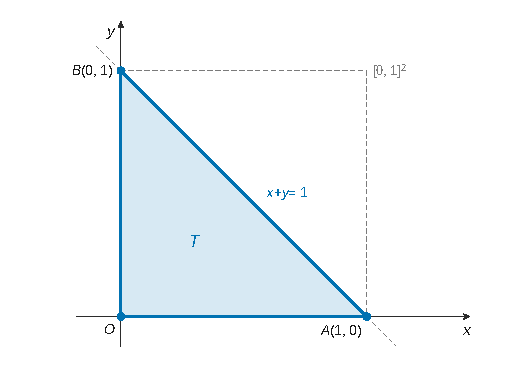
\includegraphics{figures/q4-1-triangle-t.pdf}
\caption*{Figure 1 --- Le triangle T, de sommets O(0, 0), A(1, 0), B(0, 1), bord
compris}
\end{figure}

\begin{piege}

Le domaine est un triangle, ni un carré, ni un disque, ni un demi-plan : le rapport 2026 (p.~12) décrit sur ce tracé un « bestiaire assez original ».

\end{piege}

\hypertarget{question-4.2}{%
\subsection{Question 4.2}\label{question-4.2}}

\begin{indication}{1}

De quelle nature est l'expression de \(f\) ?

\end{indication}

\hypertarget{solution-34}{%
\subsubsection{Solution}\label{solution-34}}

\(f\) est une fonction polynomiale des deux variables \(x\) et \(y\). Les fonctions polynomiales sont de classe \(\mathcal C^\infty\) sur \(\mathbb R^2\).

En particulier, \textbf{\(f\) est de classe \(\mathcal C^2\) sur \(\mathbb R^2\).}

\begin{piege}

La régularité des applications partielles \(x\mapsto f(x,y)\) et \(y\mapsto f(x,y)\) ne suffit pas à conclure pour \(f\), et le théorème de Schwarz ne prouve aucune régularité. L'argument attendu est « fonction polynomiale ».

\end{piege}

\begin{jury}

Rapport 2026 (p.~12) : « Beaucoup de copies calculent les dérivées partielles d'ordre 2, et comme elles sont de classes \(\mathcal C^2\), \(f\) aussi. »

\end{jury}

\hypertarget{question-4.3}{%
\subsection{Question 4.3}\label{question-4.3}}

\begin{indication}{1}

Théorème des bornes atteintes : vérifiez chacune de ses hypothèses.

\end{indication}

\hypertarget{solution-35}{%
\subsubsection{Solution}\label{solution-35}}

\(f\) est \textbf{continue} sur \(\mathbb R^2\) (4.2), donc sur \(T\).

\(T\) est non vide et borné, car inclus dans \([0,1]^2\).

\(T\) est fermé, comme intersection des demi-plans fermés \(\{x\ge0\}\), \(\{y\ge0\}\), \(\{x+y\le1\}\) et du fermé \([0,1]^2\).

D'après le théorème des bornes atteintes, une fonction continue sur une partie fermée bornée non vide de \(\mathbb R^2\) est bornée et atteint ses bornes : \textbf{\(f\) admet sur \(T\) un maximum et un minimum.}

\begin{piege}

Les points critiques et la hessienne ne disent rien de l'existence d'extrema sur un fermé : seule la continuité sur un fermé borné la garantit.

\end{piege}

\begin{jury}

Rapport 2026 (p.~12) : « Quelques candidats pensent bien au théorème « des bornes atteintes », mais en oubliant d'évoquer la continuité de la fonction \(f\). »

\end{jury}

\hypertarget{question-4.4}{%
\subsection{Question 4.4}\label{question-4.4}}

\begin{indication}{1}

Calculez les deux dérivées partielles ; attention au terme croisé.

\end{indication}

\hypertarget{solution-36}{%
\subsubsection{Solution}\label{solution-36}}

On a \(\partial_xf(x,y)=4-8x-4y\) et \(\partial_yf(x,y)=1-2y-4x\). Le gradient est le \textbf{vecteur} de ces deux dérivées partielles :

\equationajustee{\boxed{\nabla f(m)=\begin{pmatrix}4-8x-4y\\1-4x-2y\end{pmatrix}}}

\begin{jury}

Rapport 2026 (p.~12) : « Stupeur de constater que pour énormément de candidats, le vecteur gradient (pourtant outil banal en Physique) est un nombre, obtenu en additionnant les dérivées partielles. » Écrire \(\nabla f(m)=\frac{\partial f}{\partial x}+\frac{\partial f}{\partial y}\) est faux.

\end{jury}

\hypertarget{question-4.5}{%
\subsection{Question 4.5}\label{question-4.5}}

\begin{indication}{1}

Écrivez le système \(\nabla f=0\) et comparez les deux équations.

\end{indication}

\hypertarget{solution-37}{%
\subsubsection{Solution}\label{solution-37}}

Un point critique vérifierait :

\equationajustee{\begin{cases}8x+4y=4\\4x+2y=1\end{cases}}

En multipliant la seconde équation par \(2\), on obtient \(8x+4y=2\), incompatible avec \(8x+4y=4\).

Le système n'a aucune solution : \textbf{\(f\) n'a aucun point critique dans \(\mathbb R^2\), a fortiori dans l'intérieur de \(T\).}

\begin{methode}

Les deux lignes de la matrice hessienne \(\begin{pmatrix}-8&-4\\-4&-2\end{pmatrix}\) sont proportionnelles. Le système linéaire \(\nabla f=0\) est alors soit sans solution, soit à une infinité de solutions. Ici il est incompatible.

\end{methode}

\begin{piege}

L'énoncé affirme qu'il n'y a pas de point critique : en « trouver » un signale une erreur de calcul en 4.4. Le rapport 2026 (p.~3) relève des copies qui en trouvent et y calculent la hessienne.

\end{piege}

\hypertarget{question-4.6}{%
\subsection{Question 4.6}\label{question-4.6}}

\begin{indication}{1}

Étudiez le signe de \(g'\) sur \([0,1]\) ; pour le graphe, repérez le sommet et les tangentes aux extrémités.

\end{indication}

\hypertarget{solution-38}{%
\subsubsection{Solution}\label{solution-38}}

\(g(x)=x-x^2\) est dérivable sur \(\mathbb R\), avec \(g'(x)=1-2x\).

\(g'\) est positive sur \([0,\frac12]\) et négative sur \([\frac12,1]\). \(g\) est donc strictement croissante sur \([0,\frac12]\) et strictement décroissante sur \([\frac12,1]\).

Valeurs remarquables : \(g(0)=g(1)=0\) et \(g(\frac12)=\frac14\).

\begin{longtable}[]{@{}llllll@{}}
\toprule\noalign{}
\(x\) & \(0\) & & \(\frac12\) & & \(1\) \\
\midrule\noalign{}
\endhead
\bottomrule\noalign{}
\endlastfoot
\(g'(x)\) & \(1\) & \(+\) & \(0\) & \(-\) & \(-1\) \\
\(g(x)\) & \(0\) & croissante & \(\frac14\) & décroissante & \(0\) \\
\end{longtable}

Représentation graphique : arc de parabole tourné vers le bas, symétrique par rapport à la droite \(x=\frac12\) (figure 2).

\begin{figure}[H]
\centering
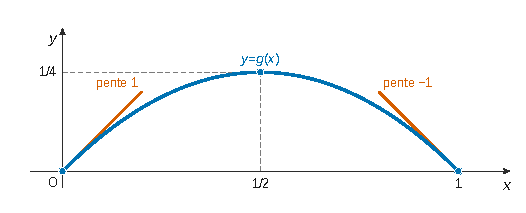
\includegraphics{figures/q4-6-graphe-g.pdf}
\caption*{Figure 2 --- Graphe de g : x ↦ x(1 − x) pour 0 ⩽ x ⩽ 1, en repère
orthonormé, maximum 1/4 en 1/2, tangentes de pentes 1 et −1 aux
extrémités}
\end{figure}

En particulier, \(0\le g(x)\le\frac14\) pour \(x\in[0,1]\).

L'égalité de gauche n'a lieu qu'en \(0\) et \(1\), celle de droite qu'en \(\frac12\).

\begin{jury}

Rapport 2026 (p.~12) : « Le tracé et l'étude de cette fonction simple pose souvent problème. On voit souvent un triangle au lieu d'une parabole. » Le graphe est un arc de parabole, à tangentes de pentes \(1\) et \(-1\) aux extrémités.

\end{jury}

\hypertarget{question-4.7}{%
\subsection{Question 4.7}\label{question-4.7}}

\begin{indication}{1}

Commencez par expliquer pourquoi les extrema ne peuvent pas être atteints à l'intérieur de \(T\).

\end{indication}

\begin{indication}{2}

Paramétrez chacun des trois côtés du triangle par une seule variable dans \([0,1]\) : vous devez retrouver la fonction \(g\) de la question précédente, éventuellement multipliée par une constante.

\end{indication}

\hypertarget{solution-39}{%
\subsubsection{Solution}\label{solution-39}}

\emph{Localisation des extrema.} L'intérieur \(\mathring T=\{x>0,\ y>0,\ x+y<1\}\) est un ouvert.

Si un extremum de \(f\) sur \(T\) était atteint en un point de \(\mathring T\), ce serait un extremum local de \(f\) sur cet ouvert, donc un point critique (condition nécessaire du premier ordre). C'est exclu par 4.5.

Les extrema de \(f\) sur \(T\), qui existent d'après 4.3, sont donc atteints sur le bord de \(T\), réunion des trois côtés.

\emph{Étude sur les côtés.}

\begin{itemize}
\tightlist
\item
  Côté \([OB]\) : \(x=0\), \(y\in[0,1]\), et \(f(0,y)=y-y^2=g(y)\).
\item
  Côté \([OA]\) : \(y=0\), \(x\in[0,1]\), et \(f(x,0)=4x-4x^2=4g(x)\).
\item
  Côté \([AB]\) : \(y=1-x\), \(x\in[0,1]\), et le calcul suivant.
\end{itemize}

\equationajustee{\begin{aligned}
f(x,1-x)&=4x+(1-x)-4x^2-(1-2x+x^2)-4x(1-x)\\
&=x-x^2\\
&=g(x).
\end{aligned}}

D'après 4.6, \(f\) prend ses valeurs dans \([0,\frac14]\) sur \([OB]\) et \([AB]\), et dans \([0,1]\) sur \([OA]\).

La valeur \(1\) n'est atteinte qu'au milieu \((\frac12,0)\) de \([OA]\). La valeur \(0\) n'est atteinte qu'aux extrémités des côtés, c'est-à-dire aux trois sommets. Donc :

\equationajustee{\boxed{\max_Tf=f\!\left(\tfrac12,0\right)=1}}

\equationajustee{\boxed{\min_Tf=0,\ \text{atteint exactement en }(0,0),\ (1,0),\ (0,1)}}

\begin{figure}[H]
\centering
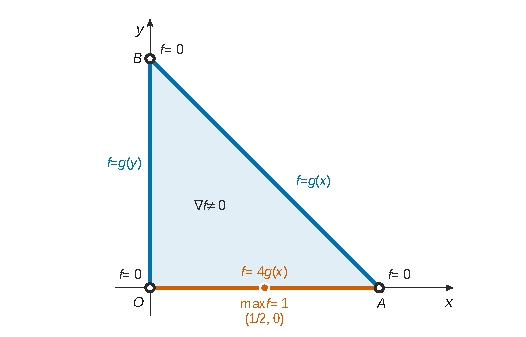
\includegraphics{figures/q4-7-bord-triangle.pdf}
\caption*{Figure 3 --- Restriction de f aux trois côtés de T : maximum 1 en (1/2,
0), minimum 0 aux sommets}
\end{figure}

\begin{piege}

Il faut étudier les \textbf{trois} côtés, y compris l'hypoténuse \(x+y=1\), et comparer les valeurs obtenues. Oublier un côté peut faire manquer un extremum.

\end{piege}

\begin{methode}

Schéma général pour les extrema d'une fonction continue sur un compact : existence par les bornes atteintes, recherche des points critiques intérieurs, étude de la restriction au bord, puis comparaison de toutes les valeurs candidates.

\end{methode}

\begin{jury}

Rapport 2026 (p.~12) : « La question (facile) est assez peu abordée et pas toujours avec les précisions attendues. » Les précisions attendues sont la justification « pas d'extremum intérieur » et les points où chaque extremum est atteint.

\end{jury}

\hypertarget{question-5}{%
\subsection{Question 5}\label{question-5}}

\begin{indication}{1}

Traduisez les contraintes sur \((p_1,p_2,p_3)\) en une condition sur \((p_1,p_2)\), et revenez à la question 3.

\end{indication}

\hypertarget{solution-40}{%
\subsubsection{Solution}\label{solution-40}}

Les conditions « \(p_1,p_2,p_3\in[0,1]\) et \(p_1+p_2+p_3=1\) » équivalent à « \((p_1,p_2)\in T\) et \(p_3=1-p_1-p_2\) ».

En effet, si \((p_1,p_2)\in T\), alors \(p_3=1-p_1-p_2\in[0,1]\), et réciproquement.

Toute loi sur \(\{1,2,3\}\) correspond donc à un point de \(T\), et \(\mathbb V(X)=f(p_1,p_2)\) (question 3). D'après 4.7 :

\begin{itemize}
\tightlist
\item
  \textbf{\(\mathbb V(X)\) est maximale, égale à \(1\), si et seulement si \((p_1,p_2,p_3)=(\frac12,0,\frac12)\)} ;
  \(X\) vaut alors \(1\) ou \(3\) avec probabilité \(\frac12\) chacune ;
\item
  \textbf{\(\mathbb V(X)\) est minimale, égale à \(0\), si et seulement si \((p_1,p_2,p_3)\in\{(1,0,0),(0,1,0),(0,0,1)\}\).}
\end{itemize}

\begin{methode}

Le résultat est intuitif : la variance mesure la dispersion, maximale quand la masse est répartie à parts égales sur les deux valeurs extrêmes. On retrouve d'ailleurs \(\mathbb V(X)=\bigl(\frac{3-1}{2}\bigr)^2=1\).

\end{methode}

\begin{jury}

Rapport 2026 (p.~12) : « Quelques tentatives mais une résolution claire et nette du problème est rarissime. » Rédigez la conclusion en termes de lois \((p_1,p_2,p_3)\), pas seulement de points de \(T\).

\end{jury}

\hypertarget{question-6}{%
\subsection{Question 6}\label{question-6}}

\begin{indication}{1}

Regardez la loi de \(X\) dans chacun des trois cas obtenus.

\end{indication}

\hypertarget{solution-41}{%
\subsubsection{Solution}\label{solution-41}}

Dans chacun des trois cas, l'un des \(p_k\) vaut \(1\) et les deux autres sont nuls.

\textbf{\(X\) est presque sûrement constante} (égale à \(1\), \(2\) ou \(3\)) : c'est une variable quasi-certaine.

C'est conforme à la propriété générale : \(\mathbb V(X)=0\) si et seulement si \(X=\mathbb E(X)\) presque sûrement.

\begin{piege}

Dire « \(X\) est constante » est un abus : \(X\) peut prendre d'autres valeurs sur un ensemble de probabilité nulle. La formulation correcte est « presque sûrement constante ».

\end{piege}

\begin{jury}

Rapport 2026 (p.~12) : « Rappelons que d'une façon générale, la variance d'une variable aléatoire est positive et s'annule pour une variable quasi-certaine. » Le jury a lu « la variance est minimale et vaut \(-4\) » : une variance négative doit alerter.

\end{jury}

\hypertarget{bilan}{%
\section{Bilan}\label{bilan}}

\textbf{Ce qui a fait la différence en 2026.} D'après le rapport, les points se sont joués sur des notions de base : définition d'un vecteur propre, rang, automorphisme, dérivée de \(x\mapsto\int_a^xh\), vecteur gradient, étude de \(x\mapsto x(1-x)\).

Les questions de synthèse (Ex. 1, Q7, Q9, Q10 ; Ex. 2, Q6.2.2, Q6.2.3 ; Ex. 3, Q5, Q6) ont été rarement menées au bout. Elles ne demandaient pourtant que d'enchaîner des résultats déjà établis.

\textbf{Méthodes à retenir.}

\begin{itemize}
\tightlist
\item
  \emph{Antisymétrie} (\(M^\top=-M\)) : déterminant nul en taille impaire ; \((f(x)\mid x)=0\), d'où un spectre réel réduit à \(\{0\}\) ; \(f^2\) symétrique à valeurs propres négatives ; \(\operatorname{Ker}f\) et \(\operatorname{Im}f\) supplémentaires orthogonaux.
  La réduction obtenue (droite noyau et plans stables sur lesquels \(f^2=\lambda\,\mathrm{Id}\), \(\lambda<0\)) est le modèle de la réduction des matrices antisymétriques réelles.
\item
  \emph{Familles libres} : pour montrer que \((x,f(x))\) est libre, on suppose une relation et l'on distingue selon le coefficient de \(f(x)\). Pour recoller deux familles libres, on utilise une somme directe.
\item
  \emph{Intégrales dépendant d'un paramètre dans les bornes} : se ramener à une primitive \(H\) et dériver \(H(v(x))-H(u(x))\). Un changement de variable \(u=x+t\) fait passer le paramètre de l'intégrande dans les bornes.
\item
  \emph{Relation de récurrence télescopique} : diviser par le bon facteur (\((-x)^k\)) pour obtenir \(u_k-u_{k-1}=a_k\), puis sommer.
\item
  \emph{Fonction constante} : dériver sur un intervalle ; une combinaison bien choisie évite tout calcul explicite.
\item
  \emph{Extrema sur un compact} : bornes atteintes, points critiques intérieurs, étude du bord, comparaison.
\end{itemize}

\textbf{Prérequis à revoir.} Définition d'un vecteur propre (non nul) ; théorème du rang ; caractérisation d'un endomorphisme symétrique par sa matrice en base orthonormale ; théorème spectral ; théorème fondamental de l'analyse ; prolongement par continuité ; équivalents et négligeabilité ; formule de transfert et formule de König-Huygens ; théorème des bornes atteintes et condition nécessaire d'extremum local sur un ouvert.

\textbf{Questions transposables.} Ces gestes reviennent régulièrement aux concours PC :

\begin{itemize}
\tightlist
\item
  « une matrice antisymétrique de taille impaire n'est pas inversible » ;
\item
  « un endomorphisme diagonalisable à une seule valeur propre est une homothétie » ;
\item
  « \(\operatorname{Ker}f\oplus\operatorname{Im}f\) via une intersection nulle » ;
\item
  « \(F_k+xF_{k-1}=\frac1k\) » (même technique pour \(\int_0^1\frac{t^n}{1+t}dt\) et le développement de \(\ln2\)) ;
\item
  « extrema d'une fonction polynomiale de degré \(2\) sur un triangle ».
\end{itemize}

\end{document}
